\documentclass[a4paper, twocolumn]{article}

% Included packages ---------------------------------------------------------- %
\usepackage{lipsum}                          % Generate random, blind, filler-text.
\usepackage[utf8]{inputenc}                  % utf-8 encoding, æ, ø , å, etc.
\usepackage{a4wide}                          % Adjust margins to better fit A4 format.
\usepackage{array}                           % Matrices.
\usepackage{dsfont}                          % Math symbols.
\usepackage{amsmath}                         % Math symbols, and enhanced matrices.
\usepackage{amsfonts}                        % Math fonts.
\usepackage{amssymb}                         % Additional symbols.
\usepackage{mathrsfs}                        % Most additional symbols.
\usepackage[pdftex]{graphicx}                % Improved inclusion of .pdf-graphics files.
\usepackage{sidecap}                         % Floats with captions to the right/left.
\usepackage{enumerate}                       % Change counters (arabic, roman, etc.).
\usepackage{floatrow}                        % Multi-figure floats.
\usepackage{subfig}                          % Multi-figure floats.
\usepackage{bm}                              % Bolded text in math mode.
\usepackage[framemethod=default]{mdframed}   % Make boxes.
\usepackage{listings}                        % For including source code.
\usepackage{mathtools}                       % Underbrackets, overbrackets.
\usepackage[dvipsnames]{xcolor}              % Colors.
\usepackage{capt-of}                         % Caption things which are not floats.
\usepackage{algorithm2e}                     % Algorithm non-float which we can caption by \captionof{algocf}{<caption>}.
\usepackage{fontawesome}                     % Github icon, etc. \faGithub
\usepackage{sidecap}                         % Floats with captions on the side.
\usepackage{tabularx}                        % Tables and stuff.
\usepackage{tabulary}                        % Tables and stuff.
\usepackage[sf,sl,outermarks]{titlesec}      % Change fonts in section{}, subsection{}, etc.
\usepackage[subfigure]{tocloft}              % Change spacing between numbers and titles in TOC.
\usepackage{pgfplots}                        % Making Tikz plots.
\usepackage{booktabs}                        % \toprule, \midrule, etc. for tables.
\usepackage{siunitx}                         % Allows S table column, aligning on decimal point.
\usepackage{chngcntr}                        % Change counter behaviour, supress increment of sub counters.
\usepackage{tikz}                            % Draw complicated pictures in a super hard way.
\usepackage{cuted}                           % Place long equations in @twocolumn over entire page.
\usepackage[version=4]{mhchem}               % Chemical reaction equations using \ce{...}.
\usepackage[%                                % Adds functionality to captions.
  tableposition = top,
  labelsep      = period,
  justification = raggedright,
  format        = hang,
  ]{caption}                                 
\usepackage[%                                % Interactive references and links, colored.
  colorlinks  = true,
  linkcolor   = black,
  urlcolor    = blue,
  citecolor   = black,
  linktocpage = true,
  ]{hyperref}            
\usepackage[%                                % References, in super-script form.
  autocite    = superscript,
  backend     = biber,
  sortcites   = true,
  style       = numeric-comp,
  sorting     = none,
  url         = false,
  ]{biblatex}
\usepackage[autostyle, english = american]{csquotes} % Assure quotation marks are inserted correctly aligned left/right.
\MakeOuterQuote{"}

% Package settings ----------------------------------------------------------- %
\renewcommand{\thesection}{\Roman{section}}         % I, II, III, IV, etc. section numbering
\renewcommand{\thesubsection}{\Alph{subsection}}    % A, B, C, etc. subsection numbering
\renewcommand{\thesubsubsection}{}                  % Remove subsubsection numbering.
\floatsetup[table]{capposition=top}                 % Place table captions above the table.
\captionsetup[subfigure]{labelformat=empty}         % Remove the (a), (b), etc. tags from subfigures.
\advance\cftsecnumwidth 1.0em\relax                 % Set the spacing between section headings and titles in TOC with tocloft.
\advance\cftsubsecindent 1.0em\relax                % Set the spacing between subsection headings and titles in TOC with tocloft.
\advance\cftsubsecnumwidth 1.0em\relax              % Set the spacing between subsubsection headings and titles in TOC with tocloft.
\newcommand{\listingsfont}{\ttfamily}
\newcommand{\inlinepy}[1]{\lstinline[language={python}]{#1}}
\newcommand{\inlinecc}[1]{\lstinline[language={c++}]{#1}}
\counterwithout*{subsection}{section}               % Dont reset the subsection counter on new \section{} calls.
\renewcommand{\figurename}{FIG.}                    % Captions of figures read FIG.
\renewcommand{\tablename}{TABLE}                    % Captions of tables read TABLE 
\renewcommand{\thetable}{\Roman{table}}             % Number tables with roman numerals.
\usetikzlibrary{matrix}                             % Some tikz picture library things.
\usetikzlibrary{arrows.meta, calc, chains, positioning}
\definecolor{listingsbackgroundcolor}{rgb}{0.975,0.975,0.975}
\colorlet{shadecolor}{listingsbackgroundcolor}



% Section headings settings -------------------------------------------------- %
\titleformat{\section}[hang]  % {command}[shape]
  {\normalfont\bfseries}      % {format}
  {\thesection.}              % {label}
  {2ex}                       % {sep}
  {\centering\MakeUppercase}  % {before-code}[after-code]

\titleformat{\subsection}[hang] % {command}[shape]
  {\normalfont\bfseries}        % {format}
  {\thesubsection.}             % {label}
  {1ex}                         % {sep}
  {\centering}                  % {before-code}[after-code]

\titleformat{\subsubsection}[hang]  % {command}[shape]
  {\normalfont\bfseries}            % {format}
  {}                                % {label}
  {1ex}                             % {sep}
  {\centering}                      % {before-code}[after-code]


% References ----------------------------------------------------------------- %
\newcommand{\Fig}[1]{Fig.\ \ref{fig:#1}}
\newcommand{\fig}[1]{Fig.\ \ref{fig:#1}}
\newcommand{\eq} [1]{Eq.\ (\ref{eq:#1})}
\newcommand{\Eq} [1]{Eq.\ (\ref{eq:#1})}
\newcommand{\tab}[1]{Table \ref{tab:#1}}
\newcommand{\Tab}[1]{Table \ref{tab:#1}}

% Matrices ------------------------------------------------------------------- %
\newcommand{\mat} [2]{\begin{matrix}[#1] #2 \end{matrix}}    % Nothing enclosing it.
\newcommand{\pmat}[2]{\begin{pmatrix}[#1] #2 \end{pmatrix}}  % Enclosing parentheses.
\newcommand{\bmat}[2]{\begin{bmatrix}[#1] #2 \end{bmatrix}}  % Enclosing square brackets.
\newcommand{\vmat}[2]{\begin{vmatrix}[#1] #2 \end{vmatrix}}  % Enclosing vertical bars.
\newcommand{\Vmat}[2]{\begin{Vmatrix}[#1] #2 \end{Vmatrix}}  % Enclosing double bars.

% Manually set alignment of rows / columns in matrices (mat, pmat, etc.) ----- %
\makeatletter
\renewcommand*\env@matrix[1][*\c@MaxMatrixCols c]{%
  \hskip -\arraycolsep
  \let\@ifnextchar\new@ifnextchar
  \array{#1}}
\makeatother

% figures in multicols environment ------------------------------------------- %
\newenvironment{Figure}
  {\par\medskip\noindent\minipage{\linewidth}}
  {\endminipage\par\medskip}

% Set bibliography file and path for images.
\addbibresource{../ref/project3-references.bib}
\bibliography{../ref/project3-references.bib}
\graphicspath{{../figures/}}

% Black frame with gray background ------------------------------------------ %
\definecolor{gray}{gray}{0.9}
\newmdenv[linecolor=white,backgroundcolor=gray]{grayframe}
\newmdenv[linecolor=white,backgroundcolor=shadecolor]{shadeframe}

% Title
\title{{\sc Solving partial differential equations with neural networks \\ {\large FYS-STK4155: Project 3}}}
\author{Morten Ledum, Håkon Kristiansen \& Kari Eriksen \\ \faGithub \ {\small \href{https://github.com/mortele/FYS-STK4155/tree/master/project3}{github.com/mortele/FYS-STK4155}}}
% ---------------------------------------------------------------------------- %
% ---------------------------------------------------------------------------- %
\begin{document}

\onecolumn
\maketitle

\begin{abstract}
\lipsum[1]
\end{abstract}

\twocolumn
\onecolumn

\tableofcontents 
\twocolumn


\section{Introduction}
\lipsum[1]

\section{Theory}
\lipsum[2]

\subsection{The heat equation}
The heat equation is a partial differential equation (in space $x$ and time $t$) which describes the evolution of temperature differences in a region of space over a time interval. It is based on \textit{Fourier's law}; the rate of heat flow through a surface is proportional to the temperature gradient across the surface, i.e.\
\begin{align}
\mathbf{q}=-k\nabla T = -k \frac{\partial T}{\partial x},
\end{align}
where $\mathbf{q}$ denotes the heat flux density, $k$ is the thermal conductivity of the surface material, and $T$ represents the temperature. Changes in temperature are proportional to changes in internal energy, with the proportionality constant being the specific heat capacity $c_p$. With the arbitrary energy zero point placed at absolute zero, this can be written as
\begin{align}
Q = c_p \rho T,
\end{align}
with $Q$ being the internal energy and $\rho$ denoting the mass density. This is essentially just a restatement of (a shifted) \textit{first law of thermodynamics}, in the absence of applied work. The total heat energy contained in a region $[a,b]$ is given by the integral
\begin{align}
\int_a^b\mathrm{d}x\,c_p\rho T(x,t).
\end{align}
Integrating over a small region of space and considering the change in internal energy over a short time interval (assuming $c_p$ and $\rho$ are both time-independent and spatially homogenous) gives 
\begin{align}
\Delta Q=& c_p \rho\int_{x}^{x+\Delta x}\mathrm{d}\chi\,\Big[T(\chi,t+\Delta t) - T(\chi,t)\Big] \nonumber \\
&= c_p\rho \int_x^{x+\Delta x}\mathrm{d}\chi\int_{t}^{t+\Delta t}\mathrm{d}\tau\,\frac{\partial T}{\partial \tau}. \label{eq:energy1}
\end{align}
Over a short time period $\Delta t$, the change in internal energy of a short segment of length $\Delta x$  must be entirely due to the heat flux in/out of the boundaries,
\begin{align}
\Delta Q &= k\int_t^{t+\Delta t}\mathrm{d}\tau\,\left[\frac{\partial T(x+\Delta x,\tau)}{\partial x} - \frac{\partial T(x,\tau)}{\partial x} \right] \nonumber \\
%
&= k\int_t^{t+\Delta t}\mathrm{d}\tau\int_x^{x+\Delta x}\mathrm{d}\chi\,\frac{\partial^2 T}{\partial \chi^2}. \label{eq:energy2}
\end{align}
By conservation of energy, the difference between \eq{energy1} and \eq{energy2} must obviously vanish. Since we are integrating over the same spatial and temporal regions in both equations, this means that the integrand must vanish identically:
\begin{align}
\frac{k}{c_p\rho} \frac{\partial^2 T}{\partial x^2} = \frac{\partial T}{\partial t}. \label{eq:heat}
\end{align}
This is known as the \textit{heat equation} and is a special case of the more general diffusion equation. 

\subsection{Closed form solution}
The 1D heat equation may be solved by applying a separation of variables ansatz, i.e.\ we assume the solution $u(x,t)$ takes the form
\begin{align}
u(x,t) = X(x)T(t), 
\end{align}
with $X(x)$ carrying all the $x$-dependence, and $T(t)$ carrying the corresponding time dependence. Introducing the compact notation 
\begin{align}
u_{x} \equiv \partial_x u =  \frac{\partial u}{\partial x}, \ \ \text{ and } \ \ u_t \equiv \partial_t u =  \frac{\partial u}{\partial t}, 
\end{align}
we find by insertion of the ansatz into \eq{heat}:
\begin{align}
\alpha^2\, u_{xx} &= u_t \nonumber \\
%
\alpha^2\, \partial_x \Big[\partial_x  X(x)T(t) \Big] &= \partial_t X(x)T(t) \nonumber \\
%
\alpha^2\, \partial_x \Big[ X_x T + XT_x \Big] &= X_tT+XT_t \nonumber \\
%
\alpha^2\, \Big[X_{xx}T + 2X_xT_x + XT_{xx}\Big]&= XT_t \nonumber \\
\frac{1}{X(x)} \frac{\partial^2 X(x)}{\partial x^2} &= \frac{1}{\alpha^2\,T(t)}\frac{\partial T(t)}{\partial t},
\end{align}
where we defined $\alpha^2\equiv k/c_p\rho$ and used the fact that $X_t=T_x=0$. As the left hand side is independent of $t$ and the right hand side is independent of $x$, the equality can only be achieved if both sides are constant. This reduces the original partial differential equation into a set of two ordinary differential equations 
\begin{align}
\frac{1}{X(x)}\frac{\partial^2X(x)}{\partial x^2}&=k  \label{eq:X(x)}\\
%
\frac{1}{\alpha^2\,T(t)}\frac{\partial T(t)}{\partial t}&=k, \label{eq:T(t)}
\end{align} 
with $k$ an undetermined constant. 

Depending on the value of $k$, the spatial part has solutions $X(x)=Ax+B$ (if $k=0$), $X(x)=A\mathrm{e}^{\mu x}+B\mathrm{e}^{-\mu x}$ (if $k=\mu^2>0$), or $X(x)=A\mathrm{e}^{\mathrm{i}\mu x}+B\mathrm{e}^{-\mathrm{i}\mu x}$ (if $k=-\mu^2<0$). The temporal equation has solutions $T(t)=C$ (if $k=0$), or $T(t)=C\mathrm{e}^{\alpha^2\mu^2 x}$ (otherwise).

\subsubsection{Applying the boundary conditons}
In order to make progress, we need to apply the specific boundary and initial conditions. In our case, the boundaries at $x=0$ and $x=L=1$ vanish, and the initial spatial solution takes the form $u(x,t=0)=\sin \pi x$. If the $k$ constant of \eq{X(x)} vanishes, then  both constants $A$ and $B$ vanish due to the boundary conditions. The same is true if $k=\mu^2>0$. It follows that the only non-trivial solutions arise when $k=-\mu^2<0$, in which case we find (left boundary)
\begin{align}
X(0) &= A\cos \mu x + B\sin\mu x = 0 \Rightarrow A=0 \nonumber 
\end{align}
and (right boundary) 
\begin{align}
X(1) &= B\sin\mu x = 0 \Rightarrow \mu=\pi n. \nonumber 
\end{align}
This gives rise to an infinite set of equations\textemdash one for each $n$\textemdash which determine the Fourier coefficients of the initial condition $u(x,t=0)$:
\begin{align}
u(x,t=0) &= \sum_{n=1}^\infty B_n \sin (n\pi x),
\end{align}
with 
\begin{align}
B_n &= 2\int_0^1\mathrm{d}x\, u(x,t=0)\,\sin(n\pi x).
\end{align}

The temporal equation, \eq{T(t)}, can now be solved only applying the boundary conditions. With the value of $\mu$ fixed at $\mu=n\pi$, we obtain 
\begin{align}
T(t) = \mathrm{e}^{-n^2\pi^2\alpha^2 t}.
\end{align}

\subsubsection{Applying the initial condition}
Combining the $X(x)$ and $T(t)$ solutions we obtain a series representation of the solution in terms of the Fourier coefficients of the initial condition $u(x,t=0)$, in which the higher frequency modes of the initial solution decays more rapidly than the corresponding lower frequency modes,
\begin{align}
u(x,t) = \sum_{n=1}^\infty B_n \sin(n\pi x)\,\mathrm{e}^{-n^2\pi^2\alpha^2 t}. \label{eq:general}
\end{align}
It is easy to see that the steady-state solution is achieved when $u(x,t)=0$, since both boundaries (left and right) act as sinks for the initial heat energy contained in the system, and no heat is ever \textit{added}. In our case, the initial condition makes the general solution \eq{general} take on a very simple form. Applying $u(x,t=0)=\sin \pi x$, it is trivial to evaluate 
\begin{align}
B_n &= 2\int_0^1\mathrm{d}x\, \sin(\pi x)\, \sin(n\pi x) = \delta_{1n},
\end{align}
due to the orthogonality of $\sin(n\pi x)$ and $\sin(m\pi x)$. This means $B_1=1$ and $B_2,B_3,\dots = 0$,
and the full solution to \eq{heat} is given by 
\begin{align}
u(x,t)=\sin(\pi x)\,\mathrm{e}^{-\pi^2\alpha^2 t}. \label{eq:full}
\end{align}

\subsection{Explicit scheme}
One of the more simple methods in the world of solving ordinary and partial differential equation numerically is the explicit scheme. This is a method that bases itself upon using the previous value of the derivatives in order to find the new ones.
We will here derive the explicit scheme for the diffusion equation, \eq{diffusion}.
\begin{equation} \label{eq:diffusion}
\frac{\partial^2 u(x,t)}{\partial x^2} = \frac{\partial u(x,t)}{\partial t}
\end{equation}
We begin with Taylor expantion of $u(x,t)$ in $t$. 
\begin{equation*}
u(x,t + \Delta t) = u(x,t) + \Delta t u'(x,t) + \frac{1}{2} \Delta t^2 u''(x,t) + ...
\end{equation*}
Truncating the series after the first term we get an expression of the first derivative of $u$ wrt. $t$ with the truncation error $O(\Delta t)$.
\begin{equation*}
u'(x,t) = \frac{u(x,t + \Delta t) - u(x,t)}{\Delta t} + O(\Delta t)
\end{equation*}
This can be simplyfied if we rewrite the derivative of $u$ wrt. $t$ as $u_t$ and discretize.
\begin{align*}
u_t &\approx \frac{u(x_i, t_j + \Delta t) - u(x_i, t_j)}{\Delta t} \\
&\approx \frac{u_{i,j+1} - u_{i,j}}{\Delta t}
\end{align*}
This is called the forward Euler method, we move one step forward in time in the integration process using the previous step. This is the simplest version of the explicit scheme.
Now we carry out the same procedure for the spatial part.
\begin{align*}
u(x + \Delta x,t) &= u(x,t) + \Delta x u'(x,t) + \frac{1}{2} \Delta x^2 u''(x,t) \\
&+ \frac{1}{3!} \Delta x^3 u'''(x,t) + ... \\
u(x - \Delta x,t) &= u(x,t) - \Delta x u'(x,t) + \frac{1}{2} \Delta x^2 u''(x,t) \\
&- \frac{1}{3!} \Delta x^3 u'''(x,t) + ... 
\end{align*}
%\begin{align}
%\Delta x u'(x,t) &= u(x + \Delta x,t) - u(x,t) - \frac{1}{2} \Delta x^2 u''(x,t) \\
%\Delta x u'(x,t) &= -u(x - \Delta x,t) + u(x,t) + \frac{1}{2} \Delta x^2 u''(x,t)
%\end{align}
%\begin{equation*}
%u''(x,t) = \frac{u(x + \Delta x,t) - 2u(x,t) + u(x - \Delta x,t)}{\Delta x^2} + O(\Delta x^2)
%\end{equation*}
We truncate at second term in order to get the second order derivative and rewrite to simplify as before. 
\begin{align*}
u_{xx} &\approx \frac{u(x_i + \Delta x,t_j) - 2u(x_i,t_j) + u(x_i - \Delta x,t_j)}{\Delta x^2} \\
&\approx \frac{u_{i+1, j} - 2u_{i,j} + u_{i-1,j}}{\Delta x^2}
\end{align*}
This is a centered difference method as we are using both previous and latter values in space to find the new second derivative of the spatial coordinate.
Adding the two solutions into the original differential equation we get the following. 
\begin{align*}
u_t &= u_{xx} \\
u_{i,j+1} - u_{i,j} &= u_{i+1,j} - 2u_{i,j} + u_{i-1,j} \frac{\Delta t}{\Delta x^2}
\end{align*}
The full diffusion equation on discretized form can further be rewritten by putting $\beta = \Delta t / \Delta x^2$.
\begin{align*}
u_{i, j+1} &= \beta (u_{i+1,j} - 2u_{i,j} + u_{i-1,j}) + u_{i,j} \\
&= \beta (u_{i+1,j} + u_{i-1,j}) + (1 - 2\beta)u_{i,j} 
\end{align*}

\subsection{Finite difference method} \label{sect:finitediff}
The most straightforward way to solve \eq{heat} numerically is through \textit{finite difference methods}, i.e.\ discretizing time and space on a grid and Taylor expanding the solution to obtain algebraic equation sets. A multitude of different strategies and schemes exists, but we will consider the \textit{explicit forward Euler} scheme. 

The spatial region $[0,L]$ is discretized by splitting it into $N$ segments, and considering only the functional values on the points $x_i=i\Delta x$ with $i\in[0,N-1]$. We denote a function $f(x,t)$ evaluated at $x_i$ (and at time $t$) by $f_i^t=f(x_i,t)$. Considering $N$ spatial points gives a step size $\Delta x$ between each point of 
\begin{align}
\Delta x = \frac{L}{N-1}.
\end{align}
In addition, we introduce a discretization in the temporal dimension with step size $\Delta t$. 

Let us consider the Taylor expansion of a function $f(x,t)$ considered at fixed $t$, $f(x;t)$, around a spatial point $x$. We use the shorthand $h\equiv (x-a)$, and consider the expansion at a point $a\not=x$. The expansions of $f(x+h;t)$ and $f(x-h;t)$ are given by, 
\begin{align}
f(x+h) &\approx f(x) + hf'(x) + h^2f''(x), \label{eq:f(x+h)}\\
f(x-h) &\approx f(x) - hf'(x) + h^2f''(x), \label{eq:f(x-h)}
\end{align}
respectively. As $t$ is considered a fixed parameter for the moment, we supressed the second functional argument for notational brevity. The shorthand $f'(x)$ is here used to denote differentiation w.r.t.\ $x$. Note that both equations hold with equality if an overall error term proportional to $h^3$ is added on the right hand side, i.e.\ $\mathcal{O}(h^3)$. Adding Eqs. (\ref{eq:f(x+h)}) and (\ref{eq:f(x-h)}) and dividing through by $h^2$ yields
\begin{strip}
\begin{align}
f(x+h)+f(x-h) &= 2f(x) + h^2f''(x) + \mathcal{O}(h^4) \nonumber \\
%
f''(x) &= \frac{f(x+h)-2f(x)+f(x-h)}{h^2} + \mathcal{O}(h^2), \label{eq:centraldiff}
\end{align}
\end{strip}
which is the three-point central difference approximation to the second derivative. Note that the resulting error is proportional to $h^2$ because the third order contributions from Eqs. (\ref{eq:f(x+h)}) and (\ref{eq:f(x-h)})\textemdash $h^3f'''(x+h)$ and $-h^3f'''(x+h)$\textemdash cancel exactly. A corresponding temporal first order derivative approximation may be found by simply considering \eq{f(x+h)}, and considering $h$ to be a small temporal step, $x$ to be a fixed parameter, and varying $t$. This gives
\begin{align}
f'(t)&= \frac{f(t+h)-f(t)}{h}+\mathcal{O}(h), \label{eq:forwarddiff}
\end{align}
where the error term is proportional to $h^2$ when disregarding the last term on the right hand side of \eq{f(x+h)}, which gives $\mathcal{O}(h)$ after dividing through by $h$.

Let us now consider \eq{centraldiff} on the previously defined grid, and take $h=\Delta x$. In the \eq{forwarddiff} case, we define $h=\Delta t$, and equate $\alpha^2\,f''(x)$ with $f'(t)$ as in the heat equation \eq{heat}. The result can be solved for $f(x,t+\Delta t)$, i.e.\ the \textit{next} time step given that the previous step is known:
\begin{align}
\frac{f_i^{j+1} - f_i^j}{\Delta t} &= \alpha^2\frac{f_{i+1}^j - 2f_i^j + f_{i-1}^j}{\Delta x^2} \nonumber \\
%
f_i^{j+1} &= f_i^j + \beta \Big[f_{i+1}^j - 2f_i^j + f_{i-1}^j\Big], \label{eq:explicit}
\end{align}
where $f_i^j$ denotes the discretized $f(x_i,t_j)$ and 
\begin{align}
\beta\equiv\alpha^2\left(\frac{\Delta t}{\Delta x^2}\right).
\end{align}
Equation (\ref{eq:explicit}) is known as the \textit{explicit Euler} scheme, and can be solved directly for $f(x,t+\Delta t)$ since the right hand side is all known at time step $t$.


\subsection{Implicit schemes}
As noted in section \ref{sect:finitediff}, applying the forward difference approximation for the first derivative in time\textemdash derived from the Taylor expansion of a function around the point $x+h$\textemdash yields the explicit Euler scheme. However, as we will see in section \ref{sect:finitestability}, the forward method has a rather weak stability criterion which necessitates the use of very small time steps to ensure the solution remains well-behaved. 

If we instead employ a backward difference approximation in time (solving \eq{f(x-h)} for an $\mathcal{O}(h)$ approximation of the first derivative) we obtain equations sets which are stable for any combination of $\Delta x$ and $\Delta t$. This allows us to use more reasonable time steps and ultimately speeds up and improves the computed solution. 

However, using this approximation,
\begin{align}
f'(t)=\frac{f(t)-f(t-h)}{h}+\mathcal{O}(h), \label{eq:backwarddiff}
\end{align}
introduces additional complexity in that we are no longer able to simply solve for the unknown $f(x,t+\Delta t)$ in the resulting heat equation approximation. Equating Eqs. (\ref{eq:centraldiff}) and (\ref{eq:backwarddiff}) yields the \textit{implicit Euler} scheme:
\begin{align}
\frac{f_i^{j} - f_i^{j-1}}{\Delta t} &= \alpha^2\frac{f_{i+1}^j - 2f_i^j + f_{i-1}^j}{\Delta x^2} \nonumber \\
%
f_i^{j-1}&= -\beta \big[f_{i+1}^j + f_{i-1}^j\big] + \big(1+2\beta\big)f_i^j.
\end{align}
We note that the only known quantity is the left hand side $f_i^{j-1}=f(x,t-\Delta t)$, which means we must solve all the equations for every spatial point $i$ simultaneously in order to ensure they are all satisfied. This gives rise to a matrix-vector equation in the place of the single algebraic equation needed for the explicit scheme. Denoting $\gamma\equiv 1+2\beta$ we may write the equation set corresponding to the integration from $t-\Delta t$ to $t$ as
\begin{align}
A\mathbf{f}^j&=\mathbf{f}^{j-1},
\end{align}
with (zeros ommitted)
\begin{align}
A = \begin{pmatrix}
\gamma & -1 & \\
-1 & \gamma & -1 \\
 & -1 & \gamma & -1 \\
 & & &  \ddots \\
 & & & -1 & \gamma & -1 \\
 & & & & -1 & \gamma 
\end{pmatrix}
\end{align}
and
\begin{align}
\mathbf{f}^j
\begin{pmatrix}
f_0^{j} \\
f_1^{j} \\
f_2^{j} \\
\vdots \\
\mathbf{f}_N^{j}
\end{pmatrix}, \ \ \ 
f^{j-1}=\begin{pmatrix}
f_0^{j-1} \\
f_1^{j-1} \\
f_2^{j-1} \\
\vdots \\
f_N^{j-1}
\end{pmatrix} 
\end{align}
As the matrix $A$ is tri-diagonal, efficient linear scaling solution algorithms exists which circumvent the traditional solution schemes, e.g.\ LU decomposition at $\mathcal{O}(N^3)$.

\subsection{The Crank-Nicolson scheme}
\lipsum[3]

\subsection{Stability analysis \label{sect:finitestability}}
\lipsum[4]


\subsection{Finite element methods}
In the case of the finite difference approximation, the derivatives in the original partial differential equation is transformed into a set of algebraic equations by application of \textit{finite difference} approximations arising from Taylor expansions of the solution function. A fundamentally different, and somewhat more sophisticated, solution strategy entails writing the original differential equation in its \textit{weak form}. This is done by integrating the original equation multiplied by a test function $v(x)$ over the domain in question. Such a \textit{finite element} (FEM) approach is normally accompanied by a simple finite difference scheme in time when partial differential equations are considered. 

\subsubsection{Functional spaces and weak forms}
Let us consider the vector space of \textit{all} functions $f:\mathds{R}^2\rightarrow\mathds{R}$, which we will call $A(\mathds{R}^2)$. Obviously, the solution to the heat equation is contained in this space, being a real-valued function of two parameters, $x$ and $t$. However, we may consider subspaces with more useful structure than the all-encompassing $A(\mathds{R}^2)$. Assuming the initial and boundary conditions are specified in a sufficiently non-pathological way, the solution at each instant in time will be continuous across the spatial integration domain, $\Omega$. In other words, the solution (at some $\tau\ge0$) $u(x;\tau)\in C(\Omega)$: The vector space of \textit{continuous} functions $f:\Omega\rightarrow\mathds{R}$. As the heat equation involves a second spatial derivative, we might assume that the solution be twice continuously differentiable, i.e.\ $u(x;\tau)\in C^2(\Omega)$.

It turns out that demanding $u\in C^2(\Omega)$ is too strict a bound on the behavior of the solution. For example, a valid solution may be \textit{not} differentiable on a subset $S\subset\Omega$ with measure zero\footnote{A set $S\subset\mathds{R}$ of measure zeros is a set with vanishing "size," e.g.\ a finite set of \textit{points}.}, known as differentiable almost everywhere (a.e.). It is more useful to consider \textit{weakly differentiable} functions, which encompass the ordinary (strongly) differentiable functions and includes other possible solutions of partial differential equations. 

Equipping our functional space with the $L^1$ integral inner product (and the associated norm), consider now a family of functions with compact support\footnote{The support of a function $f$ is the (closure) of the set of points in the domain of $f$ for which $f(x)$ does \textit{not} vanish, i.e.\ the set $\{x\in\Omega:f(x)\not=0\}$.} $\phi\in C^\infty(\Omega)$, with $\phi(\partial\Omega)=0$, where we denote by $\partial\Omega$ the boundary of the integration domain (in one dimension, this is just the end two points). Any function $f:\Omega\rightarrow\mathds{R}$ which is bounded on $\Omega$ and thus locally integrable (in the Lebesgue sense) on $\Omega$ defines a linear functional $\Lambda_f$ on $C^\infty(\Omega)$ through
\begin{align}
\Lambda_f(\phi)\equiv \int_\Omega\mathrm{d}x\, f(x)\phi(x).
\end{align}
This integral is well defined for any $\phi\in C^\infty(\Omega)$ since $\phi(x)$ is assumed to vanish outside of a compact subset of $\Omega$. Essentially, multiplication with a well-behaved function $\phi$ and integration over $\Omega$ results in something that is more well-behaved than $f$ itself. Next, consider the functional defined by the derivative of $f$, 
\begin{align}
f'(x)\equiv \lim_{h\rightarrow0}\frac{f(x+h)-f(x)}{h}. \label{eq:limit}
\end{align}
Integrating by parts and remembering that $\phi(\partial \Omega)=0$, we find
\begin{align}
\Lambda_{f'}(\phi) &=  \int_\Omega\mathrm{d}x\, f'(x)\phi(x) \nonumber \\
%
&=  -\int_\Omega\mathrm{d}x\, f(x)\phi'(x).
\end{align}
Note carefully that the first integral is only defined if the limit exists and converges for a.e.\ $x\in\Omega$, but the last integral is defined and well-behaved for any locally integrable (bounded) function $f$. This functional exists even if \eq{limit} does not converge point wise for \textit{any} $x\in\Omega$(!).

In the spirit of this, we define the \textit{weak derivative}: The $k$-th order weak derivative of $u$ is defined as a function $v$ for which the following holds
\begin{align}
\int_\Omega \mathrm{d}x\, v(x)\phi(x) = (-1)^k \int_\Omega\mathrm{d}x\, u(x)\frac{\partial^k \phi}{\partial x^k},
\end{align}
where a factor $(-1)$ is picked up for each integration by parts. 

In defining a weak derivative, we have moved the previous demands on $f$ onto a set of test functions $\phi(x)$. Even if the demands on the functions $\phi$ are stronger than the previous demands on $f$ ($\phi\in C^\infty(\Omega)$ [infinitely continuously differentiable] as opposed to $f\in C^2(\Omega)$ [twice continuously differentiable]), it will turn out that this is easier to control when considering finite element schemes. 

The functional spaces containing functions $f:\mathds{R}^m\rightarrow\mathds{R}$ with $f$ being $k$ times weakly differentiable are called \textit{Sobolev} spaces, and denoted $H^k$. 

\subsubsection{The heat equation in variational (weak) form}
As we have seen, the solution function of the original heat equation resides in the Sobolev space $H^2(\Omega)$ of a.e.\ continuous functions on the domain $\Omega$ with weak derivatives up to and including order two. Notice that if the strong (ordinary) derivative exists, then the weak and the strong derivatives are equal. This means that $H^2(\Omega)$ is a \textit{larger} space than $C^2(\Omega)$, which is larger again than the set of infinitely continuously differentiable functions $C^\infty(\Omega)$.

Let us consider a stationary diffusion equation on the form
\begin{align}
f(x)=\partial_{xx}u(x), \label{eq:stationary}
\end{align} 
with $f(x)$ some known function. Multiplying from the left by a test function $\phi(x)\in C^\infty(\Omega)$ satisfying $\phi(\partial\Omega)=0$ and integrating over $\Omega$, before integrating by parts, yields a \textit{weak} or \textit{variational} form as
\begin{align}
\int_\Omega\mathrm{d}x\, \phi(x)f(x) &= \int_\Omega \mathrm{d}x\, \phi(x)\frac{\partial^2 u}{\partial x^2} \nonumber \\
%
&= -\int_\Omega \mathrm{d}x\, \frac{\partial \phi}{\partial x}\frac{\partial u}{\partial x} \label{eq:weak1} \\
%
\int_\Omega\mathrm{d}x\, \phi(x)f(x) &=  \int_\Omega \mathrm{d}x\, \frac{\partial^2 \phi}{\partial x^2}u(x). \label{eq:weak2}
\end{align}
Proving that a solution of the weak equation is also a solution of the strong form is non-trivial and not always possible. We will in the following take if for granted that this is possible and true, or that when it is not possible we will simply interpret the weak solution as \textit{the solution}. 

\subsubsection{Basis choice and the Galerkin method}
So far we have ostensibly only introduced a second unknown function into the problem, without gaining much besides relaxation of some demands on the solution function $u$. We will now employ the Galerkin method\textemdash introducing a basis for $\phi(x)$\textemdash and derive a set of algebraic equations which may be solved to obtain an approximation to $u$. 

In order to make the problem numerically tractable, we are now forced to choose a suitable subspace $V$ of $H^2(\Omega)$ to work in. In practice, this is done by introducing a basis $\{\psi_i(x)\}_{i=1}^n$ and letting the subspace be $V_n=\text{Span}(\{\psi_i(x)\})$. In order to simplify the resulting equations, we choose a set of piecewise differentiable functions which vanish exactly on the boundary $\partial \Omega$. One of the simplest choices are the "hat functions,"
\begin{align}
\psi_i(x)=\left\{ \begin{matrix}
0                   & x\in (-\infty, x_i-h) \\%x<x_i-h \\
\frac{x-(x_i-h)}{h} & x\in [x_i-h, x_i) \\%x_i-h\le x < x_i \\
1- \frac{x-x_i}{h}  & x\in [x_i, x_i+h) \\%x_i \le x < x_i+h \\
0                   & x\in [x_i+h, \infty)%x_i+h \le x
\end{matrix}\right. \label{eq:P1}
\end{align}
i.e.\ piecewise linear functions which are non-zero in the range $[x_i-h, x_i+h]$, increasing linearly to unity from $x_i-h$ to $x_i$, before decreasing linearly back to zero between $x_i$ and $x_i+h$. 

In general, it is numerically beneficient to introduce a spatial discretization\textemdash as done in the context of the finite difference method\textemdash and choosing a set of functions $\psi_i(x)$ which vanish on all but one of the discretized points. A convenient choice often employed is the Lagrange interpolating polynomials, of which the piecewise first degree functions \eq{P1} are an example. Introducing a discretization, we may group adjacent discretized points into what are known as \textit{elements}. In the case of the Lagrange interpolating polynomial basis, the number of points (or nodes) in each element is determined by the order of the polynomials used. We will in the following refer to the interpolating polynomial bases as P$k$-bases, with $k$ denoting the order of the piecewise polynomial functions. Equation (\ref{eq:P1}) represents P1 elements. In general, the Lagrange interpolating polynomials which vanish exactly on all points $x_i$, except for a single $x_k$ on which it takes the value unity may be written as
\begin{align}
L_k(x) &= \prod_{i\not=k}\frac{x-x_i}{x_k-x_i}.
\end{align}

Using P$k$ elements, each spatial element will contain $k+1$ nodes, of which two will coincide with nodes in the neighboring elements. Examples of P1, P2, and P3 basis functions are shown in \fig{Pk}.

\begin{figure*}[p]
\centering
\subfloat[P1]{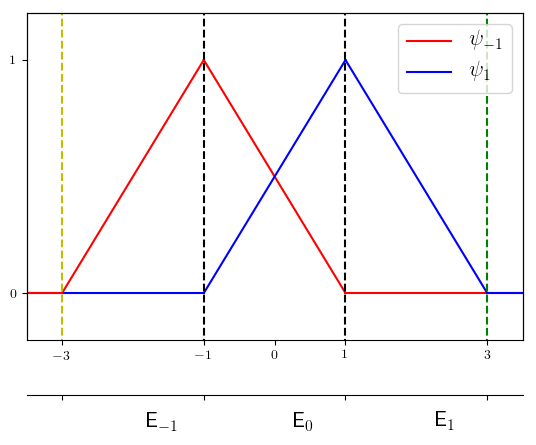
\includegraphics[width=0.4\linewidth]{P1_basis.png}}
\subfloat[P2]{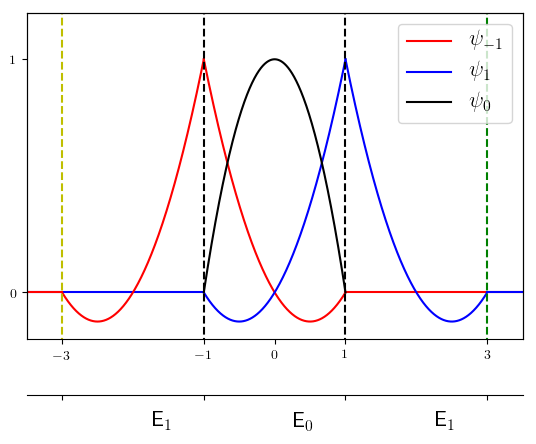
\includegraphics[width=0.4\linewidth]{P2_basis.png}} \\
\subfloat[P3]{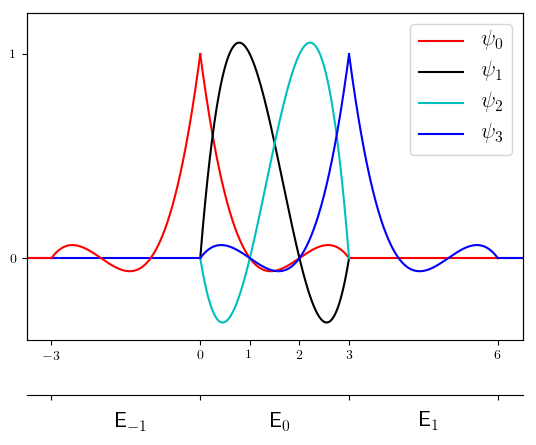
\includegraphics[width=0.5\linewidth]{P3_basis.png}}
\captionof{figure}{Piecewise Lagrange interpolating polynomial basis functions for P1, P2, and P3 elements, respectively. The basis functions $\psi_i(x)$ are labelled according to the only discretized spatial point (node) they do not vanish on. Note that all $\psi_i(x)$ take the value $\psi_i(x_i)=1$ on the one node for which they do not vanish. \label{fig:Pk}}
\end{figure*}

Working from the weak form \eq{weak1} (we may also choose to work from \eq{weak2}, but the former yields tidier mathematics), we express the arbitrary $\phi(x)$ in terms of the chosen basis functions $\{\psi_i(x)\}$. It is obvious that \textit{within the subspace }$V_n$, demanding that \eq{weak1} is satisfied \textit{for any} $\phi(x)$ is the same as demanding that it holds for any of the basis functions $\psi_i(x)$. To realize this, let us choose the arbitrary $\phi(x)$ to be $\psi_k(x)$, and express $u(x)$ in terms of its basis expansion in $\psi_i$s:
%\begin{strip}
\begin{align}
\int_\Omega\mathrm{d}x\, \psi_k(x)f(x) &= -\int_\Omega \mathrm{d}x\, \frac{\partial \psi_k}{\partial x}\frac{\partial u}{\partial x} \nonumber \\
%
\int_\Omega\mathrm{d}x\, \psi_k(x)f(x) &= -\int_\Omega \mathrm{d}x\, \sum_i c_i \frac{\partial \psi_k}{\partial x}\frac{\partial \psi_i}{\partial x}. \nonumber 
\end{align}
%\end{strip}
If we do this once for each $\psi_k$, we end up with a set of $n$ equations for the coefficients $c_i$, which determine the solution function $u(x)$ \textit{in the subspace} $V_n$. It is clear that this may be formulated in terms of a matrix-vector equation as $K\mathbf{c}=\mathbf{f}$, with
\begin{align}
K_{ij}\equiv -\int_\Omega \mathrm{d}x\, \frac{\partial \psi_i}{\partial x}\frac{\partial \psi_j}{\partial x}
\end{align}
and
\begin{align}
\mathbf{f}_i \equiv  \int_\Omega\mathrm{d}x\, \psi_i(x)f(x).
\end{align}
For smart choices of discretization, the integrals over the basis functions may be easily calculated in closed form. 

\subsubsection{Pairing the FEM method with a finite difference scheme in time}
In order to solve a time dependent problem, a finite difference scheme is traditionally introduced in the temporal dimension. In principle we may choose any such scheme, but we will in the following focus on the simplest such scheme: The forward euler (as derived in section \ref{sect:finitediff} and \eq{explicit}). Modifying the left hand side of the stationary diffusion equation\textemdash \eq{stationary}\textemdash and introducing the backwards difference approximation of \eq{backwarddiff}, we find
\begin{align}
\frac{\partial u}{\partial t} &= \alpha\frac{\partial^2 u}{\partial x^2} \nonumber \\
%
\frac{u^{n+1}-u^{n}}{\Delta t} &=  \alpha\frac{\partial^2 u^n}{\partial x^2} \nonumber \\
%
u^{n+1} &= u^{n} + \beta \frac{\partial^2 u^n}{\partial x^2}.
\end{align}
We now use the Galerkin method: Introducing a P$k$ basis $\{\psi_i(x)\}_i$, left-multiplying by $\psi_k(x)$ and integrating over $\Omega$, performing a single integration by parts on the right hand side:
\begin{strip}
\begin{align}
\int_\Omega\mathrm{d}x\, \sum_ic^{n+1}_i\psi_i(x) \psi_k(x) &= \int_\Omega\mathrm{d}x\, \sum_ic^{n}_i\psi_i(x) \psi_k(x) - \beta\int_\Omega\mathrm{d}x\, \sum_i c_i^n\frac{\partial \psi_k}{\partial x}\frac{\partial \psi_i}{\partial x}, \label{eq:FEMf}
\end{align}
\end{strip}
where superscripts denote the discretized time step, i.e.\ $u(x,t_n)=u^n(x)$. Introducing the matrix 
\begin{align}
M_{ij}\equiv \int_\Omega \mathrm{d}x\, \psi_i(x)\psi_j(x),
\end{align}
we may write \eq{FEMf} as $M\mathbf{c}^{n+1}=M\mathbf{c}^n -\beta K\mathbf{c}^n$. Note carefully that all of the right hand side is known at time step $n$, which means we may simply directly solve this equation for the coefficients of the solution function relative to the $\{\psi_i\}_i$ basis at time step $n+1$. A similar derivation yields the corresponding equation set for the \textit{backwards} Euler scheme as
\begin{align}
\Big(M +\beta K\Big)\mathbf{c}^{n+1} &= M \mathbf{c}^n. 
\end{align}


\subsection{Solving differential equations with neural networks}
A part of this project is exploring partial differential problems with the use of deep learning. Deep neural networks (DNN) are networks that consist of two hidden layers or more. In this part of the project we will be using Googles open-source library Tensorflow. A time consuming part of neural networks is the backpropagation and its equations. By using Tensorflow we avoid having to solve the derivatives of a cost function w.r.t to all the different weights and biases. It also provides us with a wast amount of applications. Different activation functions, gradients, loss function etc. And it is easy to add layers and nodes. 

In our approach on solving differential equations with DNN we will discover there are some similarities between this new method and the well known finite difference methods. For instance we will not only be using backpropagation as a way of teaching the network, we will also calculate the spatial and temporal derivatives directly, much like we do in the finite difference scheme.

However in the finite difference method we assume the problem can be rewritten into new numerical solvable equations using Taylor expansion, as mentioned above. Tensorflow uses a method called automatic differentiation (AD) to find the derivatives. 

AD is a technique for solving derivatives by recognising elementary functions $f_i$, (like addition, multiplication, exponential, trigonometric functions) which have known derivatives, within more complex functions $f$.  

\begin{equation}
f = f_1 \cdot f_2 \cdot f_3 \cdot f_4 \cdot ... \cdot f_n
\end{equation}

A composition consisting of a finite set of elementary operations for which the derivatives are known, combining the derivatives of the constituent operations through the chain rule gives the derivative of the overall composition. This is done through a process called forward and reverse mode. \eq{chain} show how we can repeatedly substitute the derivative of the inner functions in the chain rule of a function $y$ w.r.t one fixed variable $x$. In reverse mode one substitutes the outer functions in the chain rule. A computational graph showing the forward mode of $y = f(x_1, x_2) = \ln (x_1) + x_1 x_2 - \sin (x_2)$ is given in \fig{autodiff}.

Calculating the gradients of $u$ with AD gives more accurate results than using Taylor expansion approximations, which is the reason Tensorflow uses AD. In theory, AD should yield exact derivatives to numerical precision (since each step in the chain rule differentiation is exact).

\begin{strip}
\begin{equation} \label{eq:chain}
\frac{\partial y}{\partial x} = \frac{\partial y}{\partial \omega_{n-1}} \frac{\partial \omega_{n-1}}{\partial x} = \frac{\partial y}{\partial \omega_{n-1}} \left( \frac{\partial \omega_{n-1}}{\partial \omega_{n-2}} \frac{\partial \omega_{n-2}}{\partial x} \right) = \frac{\partial y}{\partial \omega_{n-1}} \left( \frac{\partial \omega_{n-1}}{\partial \omega_{n-2}} \left( \frac{\partial \omega_{n-2}}{\partial x} \right) \right) = ...
\end{equation}
\end{strip}


\begin{figure*}
\begin{centering}
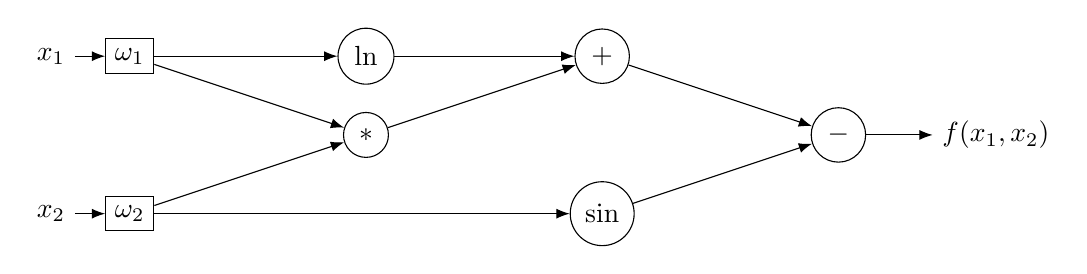
\begin{tikzpicture}[node distance=3cm, arro/.style = {-Latex}]
                                      
\tikzstyle{format} = [draw, thin]
\tikzstyle{medium} = [draw, thin, circle]

% inputs
\node at (0,-1) (x1) {$x_1$};
\node at (0,-3) (x2) {$x_2$};
% output
\node[format] at (1,-1) (w1) {$\omega_1$};
\node[format] at (1,-3) (w2) {$\omega_2$};
% connections
\draw[arro] (x1) -- (w1);
\draw[arro] (x2) -- (w2);
% output
\node[medium] at (4,-1) (ln) {$\ln$}; 
\node[medium] at (4,-2) (mult) {$*$}; 
% conections
\draw[arro] (w1) -- (ln);
\draw[arro] (w1) -- (mult);
\draw[arro] (w2) -- (mult);
% output
\node[medium] at (7,-1) (plus) {$+$};
\node[medium] at (7,-3) (sin) {$\sin$};
% connections
\draw[arro] (w2) -- (sin);
\draw[arro] (ln) -- (plus);
\draw[arro] (mult) -- (plus);
% outputs
\node[medium] at (10,-2) (minu) {$-$};
% connections
\draw[arro] (plus) -- (minu);
\draw[arro] (sin) -- (minu);
% final 
\node at (12,-2) (f) {$f(x_1, x_2)$};
% connection
\draw[arro] (minu) -- (f);
\end{tikzpicture}
\caption{A representation of the forward accumulation of $f(x_1, x_2) = \ln (x_1) + x_1 x_2 - \sin (x_2)$. We can give $\ln (\omega_1)$ a new label, $\omega_3$, and the multiplication $\omega_1 \omega_2$ we can call $\omega_4$ and so forth. Relabeling each new elementary operation and taking its derivative is the forward mode with the final varible becoming $\omega_5 = \omega_4 - \omega_3$ and $\dot{\omega_5} = \dot{y}$, the derivative of the original complex function. \label{fig:autodiff}}
\end{centering} 
\end{figure*}

We will look at a standard DNN with $n$ hidden layers called multilayer perceptron (MLP). Each layer may contain different number of neurons, or nodes. A complete description of the MLP is given in project 2 and particulary Fig. 1 is explanatory.   

Usually in supervised learning we would have one set of training data from where we computed an output and evaluated the cost function. In our case we do not have a correct output value to compare with, we are looking at a partial differential equation and our data set is simply initial values of $x$ and $t$ which we try to fit to the model. But from \eq{diff_0} we see that we seek a solution $u(x,t)$ that minimizes the right hand side of the equation. 

\begin{equation} \label{eq:diff_0}
0 = \frac{\partial u(x,t)}{\partial t} - \frac{\partial^2 u(x,t)}{\partial x^2} 
\end{equation}

It therefore makes sense to select the mean squared error (MSE) as our cost function as it allow us to do exactly so. Usually one has a set of test data to check how well the network is able to predict the outcome. However we have the exact analytical solution to check with directly.

\begin{equation}
MSE = \frac{1}{n} \sum^n \left( \frac{\partial u}{\partial t} - \frac{\partial^2 u}{\partial x^2} \right)^2
\end{equation}

Unlike finite element where we have algebraic equation sets to solve iterally, with DNN we must introduce a trial function, a guess on the solution, in order to give the network something to work on. 
Our next task is therefore designing a trial function that can be used as input for the cost function. Preferably a trial function that satisfy the initial conditions and boundary conditions and isn't to complicated. If we look at \eq{trial} we see that for $x = 0$ and $x = 1$ the trial function is zero since $\sin (0) = \sin (\pi) = 0$ which is the boundary conditions. For $t = 0$ it is $\sin(\pi x)$ which is the initial condition. And \eq{trial} fulfilles all conditions.

\begin{equation} \label{eq:trial}
u_{trial}(x,t) = (1 - t)\sin (\pi x) + x(1 - x)tN(x, t, P)
\end{equation}

The trial function is there to assure the network finds a solution that fulfilles the conditions we are given. Otherwise it could just find any function $u(x,t)$ where its first time derivative matched its second spatial derivative. $N(x,t,P)$ is a function that describes the output of the network given the $x$, $t$ and $P$, the parameters of the network (weights and biases). 

Now all we need is an optimizer in order to asjust the parameters. Tensorflow has several possible optimizer methods. However we will look at ordinary gradient descent.

\section{Results and discussion}
We now turn to the last part of this project and try to solve the diffursion equation with a neural network. We use Tensorflow to solve this problem and the structure of the network can be chenged by adding new layers in the python list called num\_hidden\_neurons, where each element is the number of nodes in each layer. Our network takes as input 100 pairs of x and t-values. These are then updated and optimized with gradient descent. 
First off the Tensorflow optimizer AdamOptimizer was tested. This method was used in project 2 giving good results. Observing an increase in the error compared to GradientDescentOptimizer however, the method was droped in this case, and gradient descent has been used through out this section.
After running the network with a number of different structures we observe that adding layers may not necessarily give better results. If we look at \tab{NN_one_layer}, just increasing the amount of nodes in a NN with one layer essentially becomes more computationally expensive. The more nodes and layers we add the more time consuming the network becomes. For 90 nodes we reach an optimal point with a maximum difference between analytical solution and the final output, $\epsilon_{diff}$, of the NN of 0.0179. 

\begin{equation}
\epsilon_{diff} = u_{analytic}(x,t) - u_{NN}(x,t,P)
\end{equation}

We try to add a new layer also containing 90 nodes. This give a better result, see \tab{NN_more_layers}. Compared to deeper networks with fewer nodes it is also better, but takes longer time than just increasing the number of iterations. Running one hidden layer containing 90 node with 200.000 iterations give a decrease in error and computational time compared to two layers with 90 nodes, see \tab{NN_90}.
It looks as though larger single layers is more important than increasing the number of layers and creating a deeper network. This is consistent with the universal approximation theorem.


\begin{strip}
\begin{center}
\captionof{table}{Simulation of NN with one hidden layer and number of neurons given in table. Number of iterations equal 100.000 and learning rate at 0.01. Results given as average over 5 runs. It is the difference between the analytical solution and the final output of the network, its maximum value and the mean, that is listed.} \label{tab:NN_one_layer} 
    \begin{tabular}{| l | l | l | l |}
    \hline
    Number of neurons & max $|\epsilon_{diff}|$ & mean $|\epsilon_{diff}|$ & Computational time [s]\\ \hline
    10 & 0.0263 & 0.00097 & 24.0 \\ \hline
    40 & 0.0420 & 0.00012 & 27.7 \\ \hline
    80 & 0.0186 & 0.00074 & 33.2 \\ \hline
    90 & 0.0179 & 0.00056 & 35.4 \\ \hline
    100 & 0.0187 & 0.00077 & 36.8 \\ 
    \hline
    \end{tabular} 
\end{center}
\end{strip}

\begin{strip}
\begin{center}
\captionof{table}{Simulation of NN with one hidden layer and 90 neurons. Number of iterations equal 200.000 and learning rate at 0.01. Results given as average over 3 runs.} \label{tab:NN_90} 
    \begin{tabular}{| l | l | l | l |}
    \hline
    Number of neurons & max $|\epsilon_{diff}|$ & mean $|\epsilon_{diff}|$ & Computational time [s]\\ \hline
    90 & 0.0113 & 0.00036 & 1m 9s \\ 
    \hline
    \end{tabular} 
\end{center}
\end{strip}

\begin{strip}
\begin{center}
\captionof{table}{Simulation of NN with the number of hidden layer and neurons given in table, [10,10] equals two layers with 10 nodes in each. Number of iterations equal 100.000 and learning rate at 0.01. Results given as average over 3 runs.} \label{tab:NN_more_layers} 
    \begin{tabular}{| l | l | l | l |}
    \hline
    [$\text{layer}_{n}$,] & max $|\epsilon_{diff}|$ & mean $|\epsilon_{diff}|$ & Computational time [s]\\ \hline
    [10,10] & 0,0844 & 0.03736 & 33.1 \\ \hline
    [10,10,10] & 0,1334 & 0,02409 & 42.0 \\ \hline
    [10,10,10,10] & 0.0156 & 0.00111 & 50.2 \\ \hline
    [90,90] & 0.0134 & 0.00098 & 1m 31s \\ 
    \hline
    \end{tabular} 
\end{center}
\end{strip}

\section{Conclusion}
\lipsum[7]


\onecolumn{
\printbibliography
}

\end{document}



